\section{System Architecture}
\label{sec:architecture}

\begin{figure*}[t]
\centering
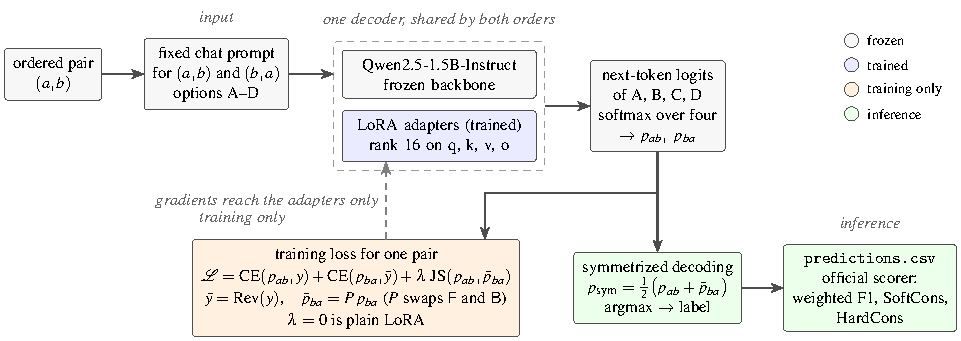
\includegraphics[width=0.8\textwidth]{figures/architecture.pdf}
\caption{Proposed system. Both orders of a pair share the tokenizer and the model weights. The backbone is frozen and only the LoRA adapters are trained. The training branch applies two supervised losses and a Jensen--Shannon consistency penalty after aligning the reversed label distribution; inference averages the aligned distributions before selecting the relation.}
\label{fig:a2-architecture}
\end{figure*}

\Cref{fig:a2-architecture} shows the flow from an ordered phrase pair to a four-way prediction and its official evaluation. The prompt presents the two phrases, in order, with the four relation options. The same Qwen2.5-1.5B-Instruct tokenizer and model process $(a,b)$ and $(b,a)$. At the answer position, the model scores the four option letters, and a softmax over these four scores gives $p_{ab}$ for the pair as given and $p_{ba}$ for the reversed pair.

The training branch applies the objective of \cref{eq:loss}: one cross-entropy term per order, plus $\lambda$ times the Jensen--Shannon divergence between $p_{ab}$ and the aligned $P\,p_{ba}$. Setting $\lambda=0$ gives the classification-only comparison system and $\lambda>0$ the consistency-aware system. At inference, the system averages the aligned distributions (\cref{eq:sym}) and writes the argmax label to \texttt{predictions.csv}, which the official scorer turns into weighted F1, \SoftCons{} and \HardCons{}.
